\themaM
\graphicspath{{../Ch8_Longueurs_et_perimetre/Images/}}

\chapter{Longueurs et\\périmètres}
\label{C07}

%%%%%%%%%%%%%%%%%%%%%%%%%%%%%%%%%%%%%%%%%%
\begin{prerequis}[Connaissances et compétences abordées]
   \begin{itemize}
      \item Distance entre deux points.
      \item Connaître le lien entre les unités de numération et les unités de mesure (exemple : dixième -> dm, centième -> cm).
      \item Notion de longueur : cas particulier du périmètre.
      \item Comparer des périmètres avec ou sans recours à la mesure (par exemple en utilisant une ficelle, ou en reportant les longueurs des côtés d’un polygone sur un segment de droite avec un compas).
      \item Calculer le périmètre d’un polygone en ajoutant les longueurs de ses côtés.
   \end{itemize}
\end{prerequis}

\vfill

\begin{debat}[Débat : le compas, un instrument de report de mesures]
   Étymologiquement le mot {\bf compas} vient du latin {\it compassare} signifiant - qui partage le même pas, la même mesure - et qui fait donc référence à un instrument qui mesure et non qui trace des cercles.
   \flushright{\it\footnotesize Source : https://compas-passion.jimdo.com}. \\
   \begin{center}
      \small
      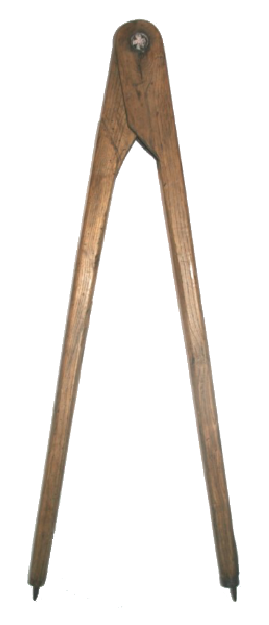
\includegraphics[height=4.5cm]{compas_simple}
      \qquad
      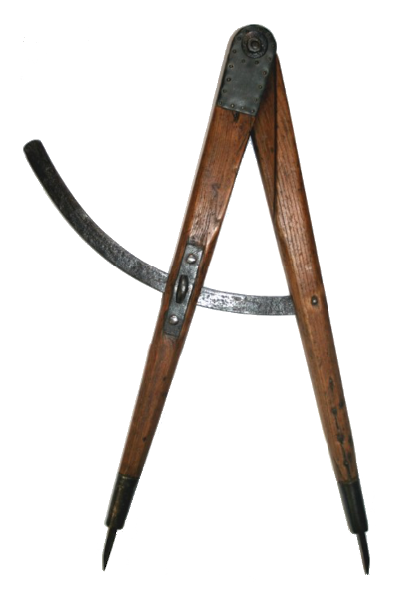
\includegraphics[height=4.5cm]{compas_secteur}
      \qquad
      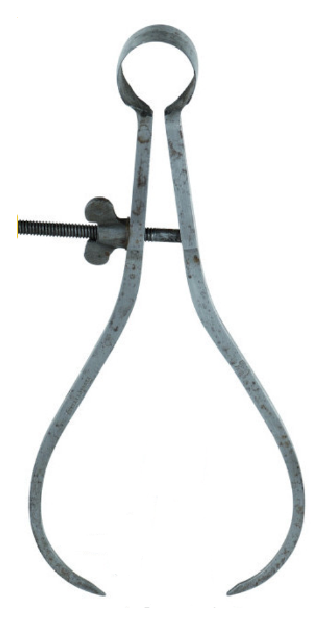
\includegraphics[height=4.5cm]{compas_epaisseur}
      \qquad
      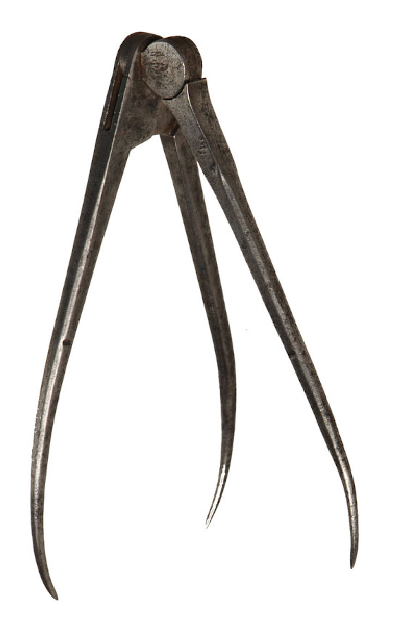
\includegraphics[height=4.5cm]{compas_3jambes} \\
      Compas simple \quad Compas à secteur courbe \; Compas d'épaisseur \quad Compas à trois jambes
   \end{center}
   \bigskip
   \begin{cadre}[B2][F4]
      \begin{center}
         Vidéo : \href{https://www.youtube.com/watch?v=gXOW4e708Hs&vl=fr}{\bf Dessin d'un cercle parfait sans outils}, chaîne YouTube de {\it Rajarts}.      \end{center}
   \end{cadre}
\end{debat}

\vfill

\textcolor{PartieGeometrie}{\large\sffamily\bfseries Cahier de compétences} : chapitre 11, exercices 1 ; 3 ; 4 ; 6 ; 23 ; 24 ; 25 ; 31 ; 37.

%%%%%%%%%%%%%%%%%%%%%%%%%%%%%%%%%%%%
%%%%%%%%%%%%%%%%%%%%%%%%%%%%%%%%%%%%%
\activites

\begin{activite}[L'art de mesurer]
   {\bf Objectifs} : mesurer une longueur et le périmètre d'un polygone avec un étalon et une règle ; comparer des méthodes, communiquer.
   \begin{QCM}
      \partie[mesurer grâce à un étalon]
         On considère la bandelette en bas de page. La découper puis donner en fonction de cette bande la mesure de la longueur d'un stylo, le périmètre du cahier de compétences et le périmètre de votre table. \\
         Écrire les résultats dans le tableau ci-dessous et comparer avec les autres élèves de la classe. \\
         
      \partie[créer une graduation]
         Avec la bandelette entière, il est difficile d'évaluer correctement les mesures demandées. Plier la bande en dix parties égales : une partie correspond donc à un dixième de bandelette. Mesurer de nouveau les trois objets cités en nombre de dixièmes de bandelette. \\
         Écrire les résultats dans le tableau ci-dessous et comparer avec les autres élèves de la classe. \\
      
      \partie[mesurer à l'aide d'une règle graduée]
         Enfin, refaire ces mesures à l'aide d'une règle graduée. \\
         Écrire les résultats dans le tableau ci-dessous et comparer avec les autres élèves de la classe. \\
         Débattre des avantages et inconvénients de chacun des outils. \\
      
      \begin{center}
         {\hautab{1.5}
         \small
         \begin{tabular}{c|C{4}|C{4}|C{4}|}
            \cline{2-4}
            & Longueur du stylo & Périmètre du cahier & Périmètre de la table \\
            \cline{2-4}
            & \begin{pspicture}(0,0.3)(4,4)
                  \pspolygon(1.8,0.5)(2.2,0.5)(2.2,3)(2,3.4)(1.8,3)
                  \psarc(2,3.4){0.06}{-120}{-70}
                  \psline(1.8,3)(1.9,2.9)(2,3)(2.1,2.9)(2.2,3)
                  \psset{linecolor=lightgray}
                  \psline(1.9,0.5)(1.9,2.9)
                  \psline(2,0.5)(2,2.98)
                  \psline(2.1,0.5)(2.1,2.9)
               \end{pspicture}
            & \begin{pspicture}(0,0.3)(4,4)
                  \psframe(1,0.5)(3,3.5)
                  \rput(2,2){\begin{minipage}{1.5cm} \footnotesize Cahier\\de\\compétences \end{minipage}}
                  \rput(2.5,3){\large 6\up{e}}
               \end{pspicture}
               & \begin{pspicture}(0,0.3)(4,4)
                     \psline(0.5,0.7)(0.5,2.5)(1.5,3.3)(3.5,3.3)(2.5,2.5)(2.5,0.7)
                     \psline(3.5,1.7)(3.5,3.3)
                     \psline(0.5,2.5)(2.5,2.5)
                     \psline(0.5,2.3)(2.5,2.3)(3.5,3.1)
                     \psline(1.5,1.7)(1.5,2.3)
                  \end{pspicture} \\
            \hline
            Avec l'étalon & & & \\
            \hline
            Etalon gradué & & & \\
            \hline
            Règle graduée & & & \\
            \hline
         \end{tabular}}
      \end{center}
      \bigskip
   \end{QCM}
   \vfill
   Bandelette à découper :
   \begin{center}
      \begin{pspicture}(0,0)(15,1.5)
         \psframe(0,0)(15,1.5)
     \end{pspicture}
  \end{center}
\end{activite}


%%%%%%%%%%%%%%%%%%%%%%%%%%%%%%%%%%%%%%
%%%%%%%%%%%%%%%%%%%%%%%%%%%%%%%%%%%%%%
\cours 

%%%%%%%%%%%%%%%%%%%%%%%%%%%%%%%%%%%%%%%%%%
\section{Le compas comme instrument de report de mesure}

\begin{methode}[Reporter une longueur au compas]
   Pour reporter la mesure de la longueur d'un segment avec un compas, prendre la longueur de ce segment en plaçant chaque pointe du compas sur l'une des extrémités du segment puis la reporter sur une autre portion de droite.
   \exercice
      Reproduire un segment $[CD]$ de même mesure que $[AB]$. \\
      \begin{pspicture}(0,0.5)(4,1.5)
         \psline[linecolor=violet]{|-|}(1,0.5)(2.8,1.4)
         \rput(1,0.1){\textcolor{violet}{$A$}}
         \rput(2.8,1){\textcolor{violet}{$B$}}
      \end{pspicture}
   \correction
      {\psset{unit=0.7}
      \begin{pspicture}(-3,0)(4.5,3.5)
         \psline[linecolor=violet]{|-|}(1,0.5)(2.8,1.4)
         \rput(1,0.1){\textcolor{violet}{$A$}}
         \rput(2.8,1){\textcolor{violet}{$B$}}
         \compas{2}{0.8}{25}{1}{18}
         \psline[linewidth=1mm]{->}(2,3.9)(4.5,3.7)
      \end{pspicture}
      \begin{pspicture}(0.5,-0.5)(4,3.5)
         \rotatebox{-27}{
            \psline(0,0)(4,2)
            \rput(1,0.1){\textcolor{cyan}{$C$}}
            \rput(2.8,1){\textcolor{cyan}{$D$}}
            \psline[linecolor=cyan]{|-|}(1,0.5)(2.8,1.4)
            \psarc[linecolor=gray!50](2.8,1.4){2}{180}{240}
            \compas{2}{0.8}{25}{1}{18}}
      \end{pspicture}}
\end{methode}




\section{Unités de longueur} %%% 1

On peut mesurer une longueur grâce au mètre (m) et à toutes les unités qui en découlent :
   \begin{center}
   \begin{CLtableau}{0.9\linewidth}{8}{p{3cm}}
      \hline
      Préfixe & kilo & hecto & déca & & déci & centi & milli \\
      \hline
      Signification & 1 000 & 100 & 10 & 1 & 1/10 & 1/100 & 1/1 000 \\
      \hline
      Unité de longueur & km & hm & dam & m & dm & cm & mm \\
      \hline
      Exemple & & $9$ & $7$ & $3$ & $2$ & $1$ & \\
      \hline
   \end{CLtableau}
   \end{center}

\begin{exemple*1}
   $\ukm{0,97321} =\uhm{9,7321} =\udam{97,321} =\um{973,21}=\udm{9732,1} =\ucm{97321} =\umm{973210}$. Pour passer d'une unité à une autre, on multiplie/divise par 10, 100, 1 000 \dots
\end{exemple*1}

\begin{definition}
   La {\bf longueur} $AB$ d'un segment [$AB$] est la distance qui sépare ses deux extrémités $A$ et $B$.
\end{definition}


%%%%%%%%%%%%%%%%%%%%%%%%%%%%%%%%%%%%%
\section{Périmètre d'un polygone}

\begin{definition}
   Le \textbf{périmètre} d'une figure est la mesure du contour de cette figure.
\end{definition}

\begin{propriete}
   Pour calculer le périmètre d'un polygone, on additionne la mesure de chacun de ses segments.
\end{propriete}

\begin{exemple}[0.5]
   {\psset{unit=0.45}
   \begin{pspicture}(-0.5,0)(11,5.5)
      \psgrid[subgriddiv=0,gridlabels=0pt,gridcolor=gray](11,5)
      \put(1,1){\pspolygon[fillstyle=solid,fillcolor=B2,linewidth=0.1](0,0)(2,0)(2,3)(0,3)(0,2)(1,2)(1,1)(0,1)(0,0)}
      \put(4,1){\pspolygon[fillstyle=solid,fillcolor=A2,linewidth=0.1](0,0)(2,0)(2,2)(1,2)(1,3)(0,3)(0,0)}
      \put(7,1){\pspolygon[fillstyle=solid,fillcolor=J2,linewidth=0.1](1,0)(2,0)(2,1)(3,1)(3,2)(2,2)(2,3)(1,3)(1,2)(0,2)(0,1)(1,1)(1,0)}
      \rput(2.5,2.4){\textbf{A}}
      \rput(5,2.4){\textbf{B}}
      \rput(8.5,2.4){\textbf{C}}
      \psline[linewidth=0.4mm]{|-|}(6,4)(7,4)
      \rput(6.5,4.6){\small$u.\ell$.}
   \end{pspicture}}
\correction
   $u.\ell$ désigne l'unité de longueur :
   \begin{itemize}
      \item le périmètre de la figure A vaut 12 $u.\ell$;   
      \item le périmètre de la figure B vaut 10 $u.\ell$;
      \item le périmètre de la figure C vaut 12 $u.\ell$
   \end{itemize} 
\end{exemple}


%%%%%%%%%%%%%%%%%%%%%%%%%%%%%%%%%%%%%%
%%%%%%%%%%%%%%%%%%%%%%%%%%%%%%%%%%%%%%
\exercicesbase

\begin{colonne*exercice}

\serie{Reporter des mesures} %%%%%%%%%%%%%%%%%%%%%%%%%%

\begin{exercice}
   Reporter la mesure de chaque segment qui compose les deux polygones sur une droite. En déduire lequel de ces deux polygones a le plus grand périmètre.
   \begin{pspicture}(0.5,0.5)(8,6.5)
      \pspolygon(1,1)(3,1)(4,5)(2,6)
      \pspolygon(5,1)(7,2)(8,3)(7,4)(5,4)(4,3)
      \rput(2.5,3.2){\large 1}
      \rput(5.9,2.8){\large2}
   \end{pspicture}
\end{exercice}

\begin{exercice}
   À l'aide d'un compas, classer ces segments du plus petit au plus grand. Vérifier ensuite en mesurant chaque segment.
   \begin{center}
   {\psset{unit=0.55}
      \begin{pspicture}(0,0)(13,10)
         \pstGeonode[PointSymbol=+,PosAngle={180,0,-100,80,130,-60,170,-10,-100,80}](1,2){A}(7,2){B}(1,4){C}(2,9){D}(7,8){E}(11,2){F}(3,5){G}(8,4){H}(12,2.5){I}(13,9){J}
         \pstLineAB{A}{B}
         \pstLineAB{C}{D}
         \pstLineAB{E}{F}
         \pstLineAB{G}{H}
         \pstLineAB{I}{J}
      \end{pspicture}}
   \end{center}
\end{exercice}


\serie{Calculer de périmètres} %%%%%%%%%%%%%%%%%%%%

\begin{exercice}
   En prenant comme unité de longueur la longueur du côté d'un carreau du cahier, réaliser trois figures différentes qui ont un périmètre de douze unités.
\end{exercice}

\medskip

\begin{exercice}
   Sachant que l'unité de longueur est la longueur d'un côté de carreau, déterminer le périmètre de chacune des figures suivantes.
   \begin{center}
      \psset{unit=0.52}
      \begin{pspicture}(0,-1.5)(15,10)
         \psgrid[subgriddiv=0,gridlabels=0,gridcolor=lightgray](0,-1)(15,10)
         \psset{linewidth=0.3mm}
         \psframe(1,1)(4,3)
         \rput(2.5,2){\ding{205}} %4
         \pspolygon(5,0)(11,0)(11,1)(10,1)(10,4)(8,4)(8,2)(5,2)
         \rput(8.5,1.5){\ding{206}} %5
         \pspolygon(1,4)(1,9)(5,9)(5,8)(2,8)(2,7)(4,7)(4,6)(2,6)(2,4)
         \rput(1.5,6.5){\ding{202}} %1
         \pspolygon(6,7)(8,7)(8,8)(11,8)(11,9)(6,9)
         \rput(7.5,8.4){\ding{203}} % 2
         \pspolygon(5,4)(5,6)(12,6)(12,8)(14,8)(14,4)(13,4)(13,2)(14,2)(14,1)(12,1)(12,2)(11,2)(11,5)(6,5)(6,5)(6,4)
         \rput(13,5.5){\ding{204}} %3
      \end{pspicture}
   \end{center}
\end{exercice}
         
\begin{exercice}
   Classer ces figures dans l'ordre croissant de leur périmètre \og au jugé \fg{} puis déterminer le périmètre de chaque figure, exprimé en unités de longueur (u.l.) et vérifier que le classement est correct.
   \begin{center}
      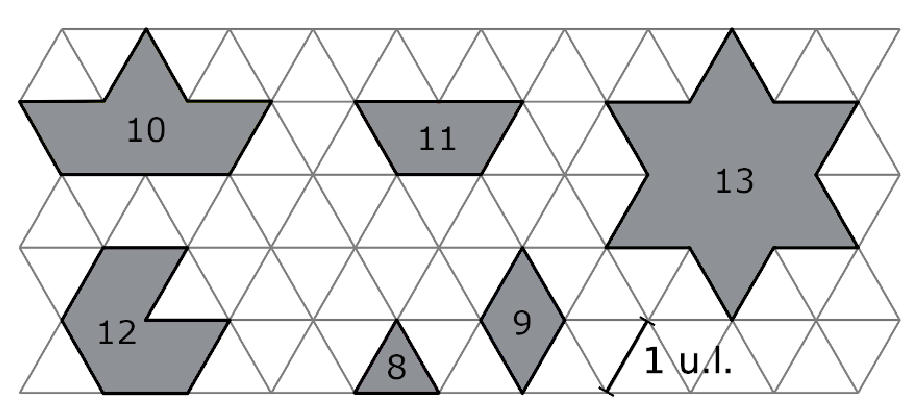
\includegraphics[width=8cm]{triangulaire}
   \end{center}
\end{exercice}

\medskip

\begin{exercice}
   Déterminer le périmètre de chaque figure en \ucm{}. \smallskip
   \begin{center}
      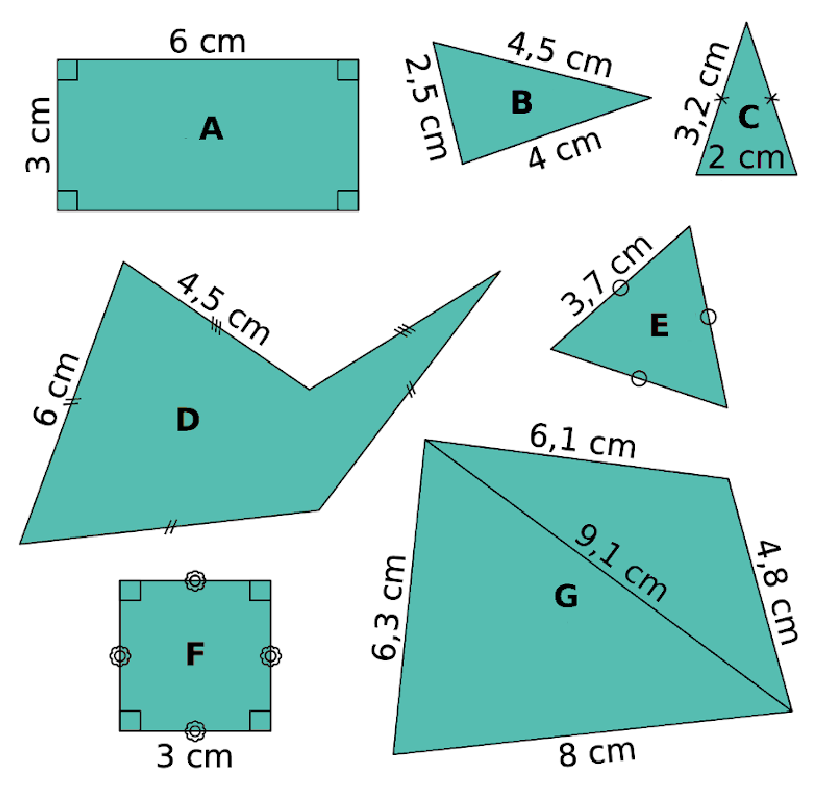
\includegraphics[width=8cm]{perimetres_divers}
   \end{center}
\end{exercice}

\hfill {\footnotesize\it Source : inspiré de Sesamath, le manuel 6\up{e}. Génération 5 - 2013}
\end{colonne*exercice}


%%%%%%%%%%%%%%%%%%%%%%%%%%%%%%%%%%%%%%%
%%%%%%%%%%%%%%%%%%%%%%%%%%%%%%%%%%%%%%%
\Recreation
   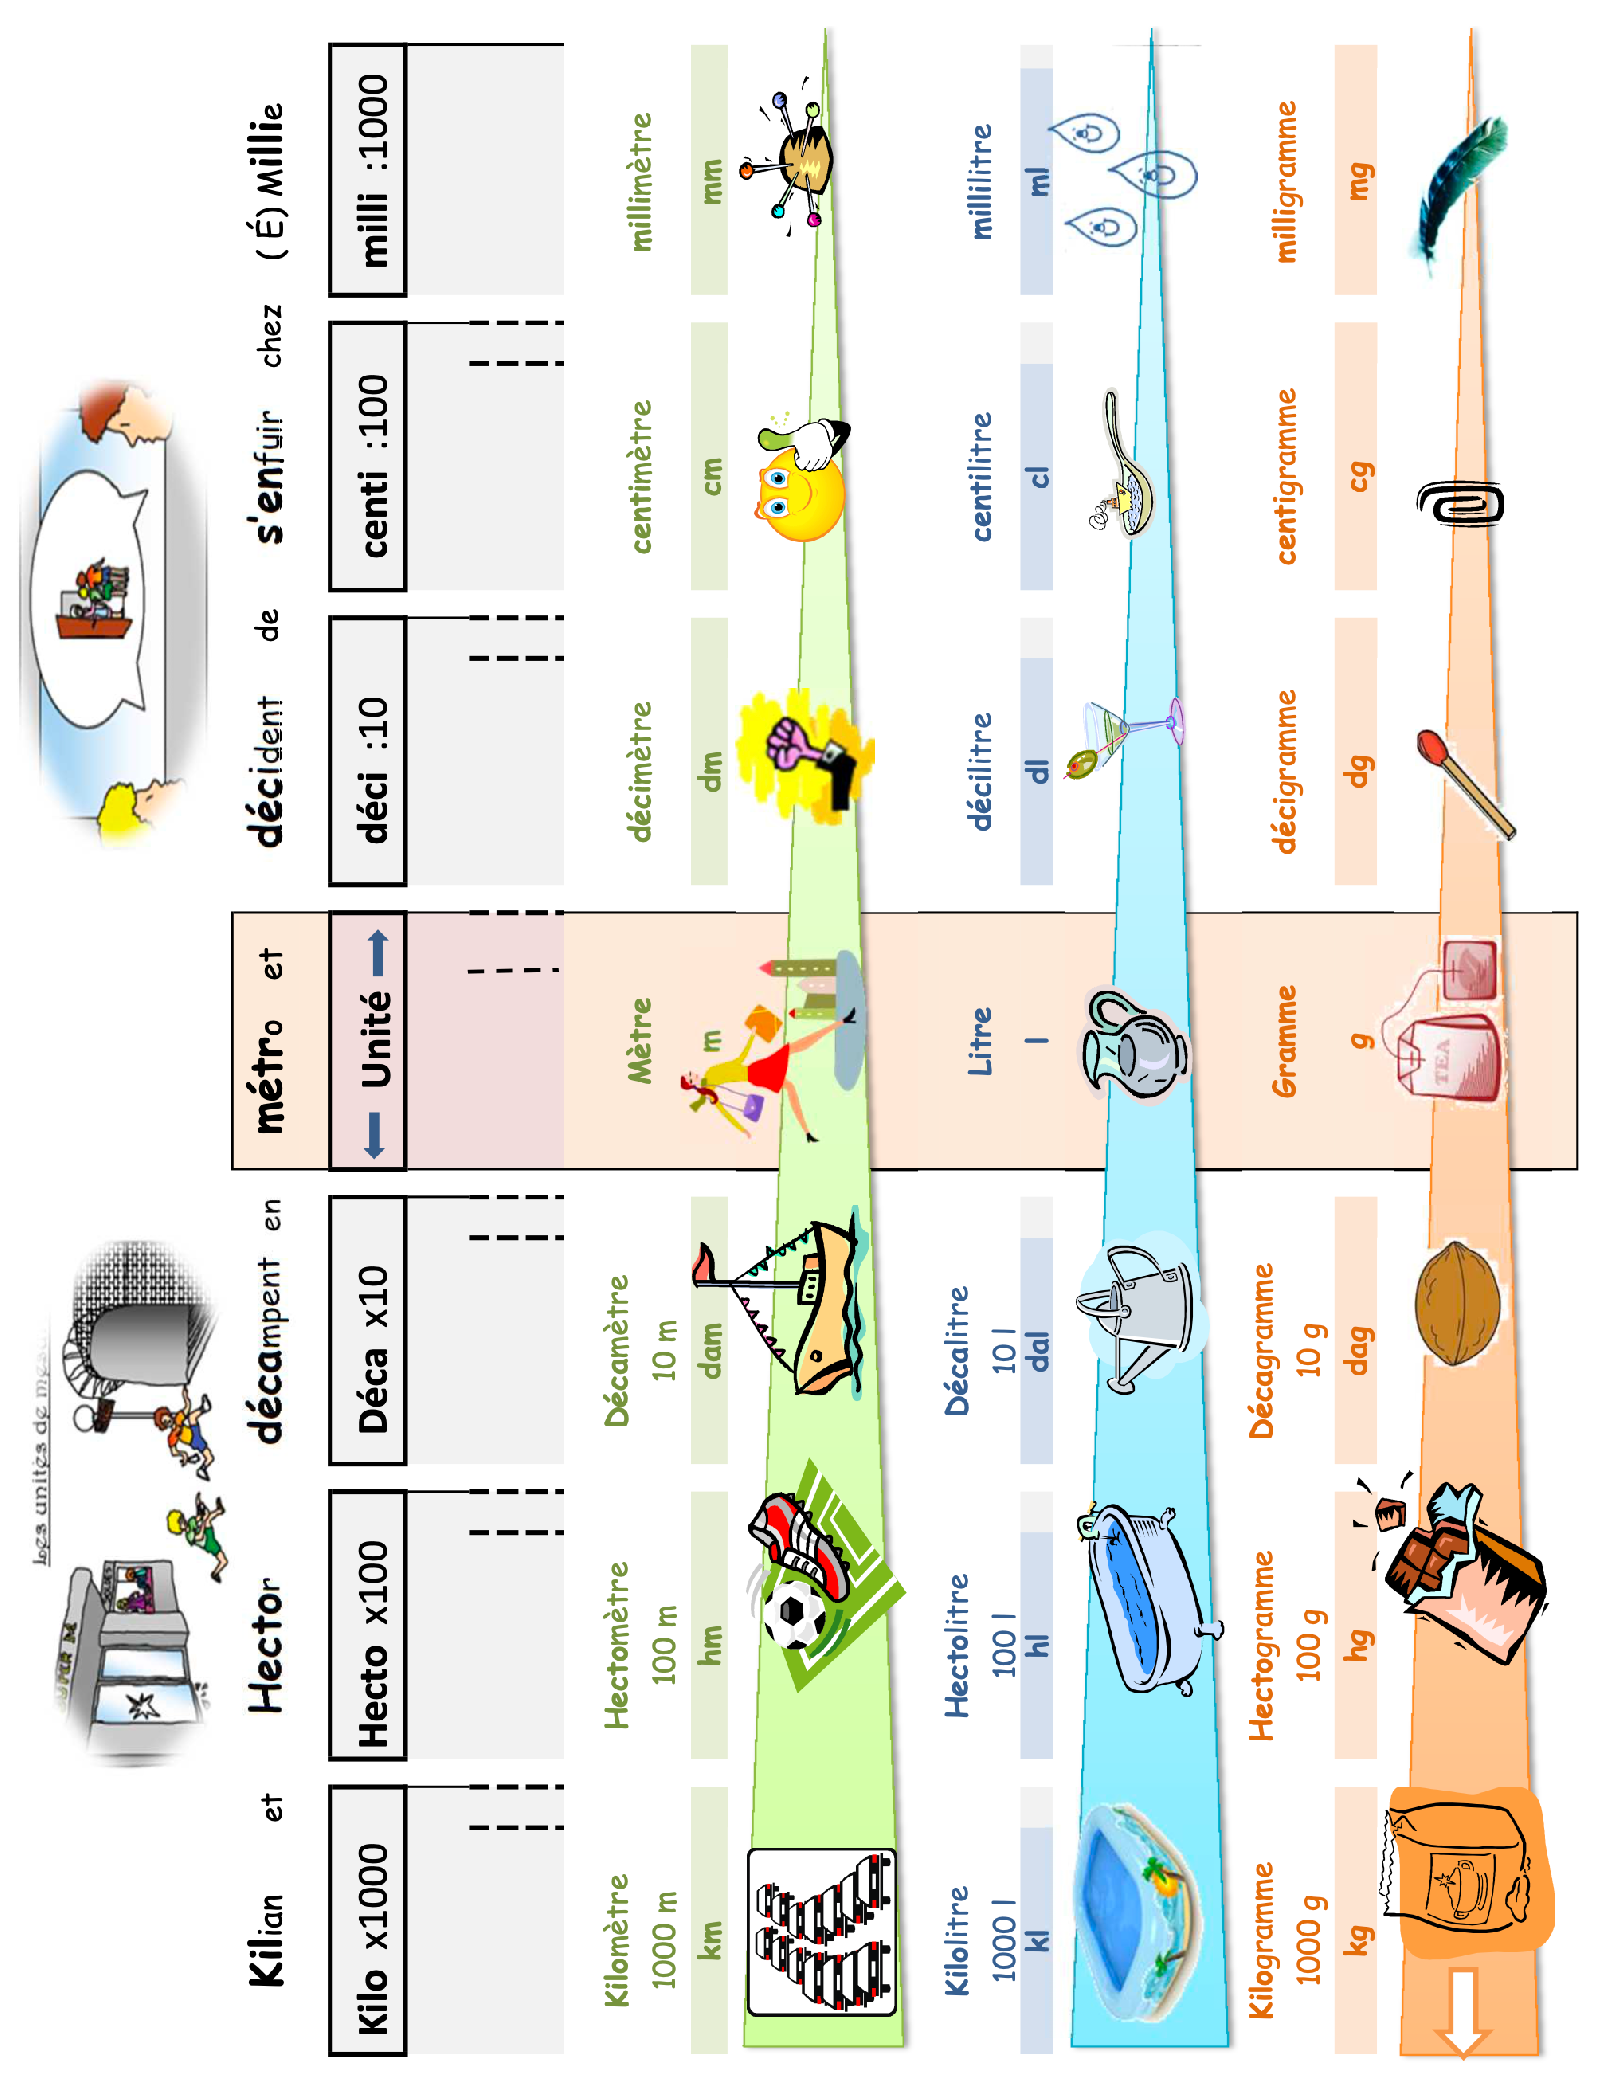
\includegraphics[width=16.6cm]{tableau_mesures}
   \begin{flushright}
      {\it\footnotesize Source : \href{https://ateliersdys.ch/les-unites-de-mesure}{Les ateliers DYS}}
   \end{flushright}

